%Version 3.1 December 2024
% See section 11 of the User Manual for version history
%
%%%%%%%%%%%%%%%%%%%%%%%%%%%%%%%%%%%%%%%%%%%%%%%%%%%%%%%%%%%%%%%%%%%%%%
%%                                                                 %%
%% Please do not use \input{...} to include other tex files.       %%
%% Submit your LaTeX manuscript as one .tex document.              %%
%%                                                                 %%
%% All additional figures and files should be attached             %%
%% separately and not embedded in the \TeX\ document itself.       %%
%%                                                                 %%
%%%%%%%%%%%%%%%%%%%%%%%%%%%%%%%%%%%%%%%%%%%%%%%%%%%%%%%%%%%%%%%%%%%%%

\documentclass[pdflatex,sn-basic]{sn-jnl}% Springer Nature basic reference style, single-column layout

%%%% Standard Packages
%%<additional latex packages if required can be included here>

\usepackage{graphicx}%
\usepackage{multirow}%
\usepackage{amsmath,amssymb,amsfonts}%
\usepackage{amsthm}%
\usepackage{mathrsfs}%
\usepackage[title]{appendix}%
\usepackage{xcolor}%
\usepackage{textcomp}%
\usepackage{manyfoot}%
\usepackage{booktabs}%
\usepackage{listings}%
\usepackage{algorithm}%
\usepackage{algpseudocode}%
\usepackage{url}%
\usepackage{array}%
\usepackage{tabularx}%
\usepackage{makecell}%
\usepackage{float}%
\usepackage[section]{placeins}%
%%%%

% Slightly loosen table rows for readability without changing body text spacing.
\renewcommand{\arraystretch}{1.16}%
\setlength{\extrarowheight}{0.6pt}%
\newcolumntype{L}[1]{>{\raggedright\arraybackslash}p{#1}}%
\newcolumntype{C}[1]{>{\centering\arraybackslash}p{#1}}%
\newcolumntype{Y}{>{\raggedright\arraybackslash}X}%
\newcolumntype{Z}{>{\centering\arraybackslash}X}%
\newcommand{\compacttable}{\scriptsize\setlength{\tabcolsep}{2.2pt}\renewcommand{\arraystretch}{1.12}}%
\makeatletter
\g@addto@macro\UrlBreaks{\do\/\do\-\do\.}%
\makeatother
\Urlmuskip=0mu plus 1mu\relax
\hypersetup{hypertexnames=false}%

% Local readability override for author-side PDF review.
% Springer Nature's class uses a narrow two-sided text block with a binding offset;
% comment this line before submission if the journal requires the untouched template layout.
\geometry{textwidth=154mm,bindingoffset=0mm}%
\usepackage{indentfirst}%

%%%%%=============================================================================%%%%
%%%%  Remarks: This template is provided to aid authors with the preparation
%%%%  of original research articles intended for submission to journals published
%%%%  by Springer Nature. The guidance has been prepared in partnership with
%%%%  production teams to conform to Springer Nature technical requirements.
%%%%  Editorial and presentation requirements differ among journal portfolios and
%%%%  research disciplines. You may find sections in this template are irrelevant
%%%%  to your work and are empowered to omit any such section if allowed by the
%%%%  journal you intend to submit to. The submission guidelines and policies
%%%%  of the journal take precedence. A detailed User Manual is available in the
%%%%  template package for technical guidance.
%%%%%=============================================================================%%%%

\theoremstyle{thmstyleone}%
\newtheorem{theorem}{Theorem}%
\newtheorem{proposition}[theorem]{Proposition}%

\theoremstyle{thmstyletwo}%
\newtheorem{example}{Example}%
\newtheorem{remark}{Remark}%

\theoremstyle{thmstylethree}%
\newtheorem{definition}{Definition}%

\lstset{
  basicstyle=\ttfamily\footnotesize,
  backgroundcolor=\color{gray!5},
  frame=single,
  keywordstyle=\color{blue}\bfseries,
  commentstyle=\color{gray}\itshape,
  stringstyle=\color{red!60!black},
  numbers=left,
  numberstyle=\tiny\color{gray},
  breaklines=true,
  captionpos=b,
  escapeinside={(*@}{@*)}
}

\raggedbottom

\begin{document}
\articletype{RESEARCH}

\title{Evidence-Guided Crash Adjudication for LLM-assisted Fuzzing of Automotive In-vehicle Open-source Software Components}

\author*[1]{\fnm{Qingguan} \sur{Gao}}\email{gaoqingguan@seu.edu.cn}

\author[1]{\fnm{Ying} \sur{Zhang}}\email{zhangying@seu.edu.cn}

\author[2]{\fnm{Letian} \sur{Sha}}\email{ltsha@njupt.edu.cn}

\affil*[1]{\orgname{School of Cyber Science and Engineering, Southeast University}, \orgaddress{\city{Nanjing}, \country{China}}}

\affil[2]{\orgname{School of Computer Science, Nanjing University of Posts and Telecommunications}, \orgaddress{\city{Nanjing}, \country{China}}}

\abstract{Connected vehicle systems rely heavily on open-source software components, which necessitates effective fuzz testing to ensure robust security validation. Driven by the advancement of Large Language Models (LLMs), fuzz-driver generation has become increasingly automated. Nevertheless, directly applying LLMs to raw crash reports can produce many false alerts, while case-by-case triage incurs prohibitive labor costs. To tackle this problem, we propose CrashSage, an evidence-guided framework for post-fuzzing crash triage in LLM-assisted fuzzing. Before final LLM analysis, CrashSage prepares crash evidence through three key designs: rule-guided crash attribution, representative selection, and crash-context reconstruction. Rule-guided crash attribution filters low-value reports and likely driver-induced crashes to improve false-alert judgment. Representative selection compares exact and stack signatures among retained reports to identify repeated crash instances and submits only selected representatives to the LLM, reducing redundant analysis. Crash-context reconstruction enriches representative crashes with static and runtime evidence, helping determine whether the faulty state comes from the generated driver or the target component. Experiments on 123 crash reports show that CrashSage improves crash attribution and reduces LLM submissions from 123 to 21 (82.9\%). These results demonstrate its effectiveness in improving crash attribution and efficiency for LLM-assisted fuzzing of connected-vehicle supply-chain components.}

\keywords{fuzz testing, crash adjudication, large language model, crash attribution, connected vehicle security}

\maketitle


\section{Introduction}
\label{sec:introduction}

Intelligent connected vehicle (ICV) systems increasingly depend on open-source supply-chain components \citep{ref1,ref2,ref3,ref4,ref32}, causing ICV software to inherit security risks from these components. To expose crash-inducing defects in such components, fuzz testing is widely adopted \citep{ref16,ref17,ref7}. Yet validating diverse supply-chain components at scale still requires a large number of component-specific fuzz drivers. Recent LLM-assisted fuzzing systems attempt to ease this bottleneck by using LLMs to synthesize fuzz drivers automatically \citep{ref8,ref9,ref10,ref11,ref12}.

LLM-assisted fuzzing differs from conventional component fuzzing, where the harness is usually written or reviewed by developers and is therefore treated as trusted during crash inspection. In LLM-assisted fuzzing, the generated driver is not necessarily a trusted harness. It invokes target-component APIs with mutated inputs, but it may omit required initialization, construct invalid arguments, or introduce harness-level memory errors. As a result, a crash report no longer reflects target-component behavior alone, but the interaction between the generated driver and the target component.

This difference leads to three challenges in false-alert judgment, crash localization, and efficiency. First, existing crash adjudication tends to treat crash reports as direct evidence of target-component-attributed crashes, leaving driver-induced false alerts difficult to distinguish from target-component-originated crashes. Second, existing adjudication lacks localization evidence that combines static code context and runtime context, which can lead to inaccurate crash attribution. Third, repeated crash instances triggered during fuzzing may stem from the same underlying failure pattern, but existing workflows still analyze them separately, resulting in redundant triage, localization effort, and LLM submissions.

To address this problem, we propose CrashSage, an evidence-guided crash-adjudication pipeline tailored for LLM-assisted fuzzing with untrusted generated drivers. Rather than reasoning directly over raw crash reports, CrashSage applies rule-guided crash attribution to filter low-value reports and likely driver-induced failures, uses representative selection to reduce repeated crash instances, and performs crash-context reconstruction to localize the origin and propagation of the faulty state for the selected representatives. The resulting evidence is then submitted to LLM analysis for final crash diagnosis. In this way, the LLM reasons over filtered, representative, and localized crash evidence. CrashSage is designed as a post-fuzzing triage aid that reduces the number of reports requiring detailed inspection and prepares attribution evidence for retained representative crashes. The main contributions of this paper are listed as follows.

\begin{itemize}
    \item \textbf{CrashSage pipeline.} We propose an evidence-guided crash-adjudication pipeline for LLM-assisted fuzzing. By preparing structured crash evidence before model reasoning, CrashSage reframes the LLM from a primary classifier over raw crash text into a final analyzer over curated execution evidence.
    \item \textbf{Rule-guided crash attribution.} We introduce rule-guided crash attribution over sanitizer signals and stack-frame roles. This stage filters low-value reports and likely driver-induced crashes before LLM analysis, mitigating over-attribution bias in prompt-based methods and improving false-alert judgment.
    \item \textbf{Representative selection.} We compare exact and stack signatures to identify repeated crash instances and retain representative crashes for subsequent LLM analysis. This selection process reduces redundant analysis while preserving the relationship between each repeated crash and its representative.
    \item \textbf{Crash-context reconstruction.} We reconstruct static code context and runtime context for representative crashes to trace a crash across driver and component code. By combining source locations with execution-state evidence, this stage supports more accurate crash attribution and root-cause localization than static code context alone.
    \item \textbf{Experimental evaluation.} We evaluate CrashSage using 123 crash reports from four representative open-source supply-chain components and report results under four external adjudicators. Compared with the baseline, the full pipeline improves precision and F1 under external adjudication and reduces end-to-end LLM submissions from 123 to 21 (82.9\%). Runtime context reconstruction and LLM analysis are the main sources of latency, while rule-guided crash attribution and representative selection each require less than 10 ms per report.
\end{itemize}

The rest of the paper is organized as follows. Section~\ref{sec:related-work} reviews related work. Section~\ref{sec:preliminaries} introduces the LLM-assisted fuzzing framework and its crash-adjudication challenges. Section~\ref{sec:approach} presents the design of CrashSage, Section~\ref{sec:evaluation} reports the evaluation, and Section~\ref{sec:conclusion} concludes the paper.


\section{Related Work}
\label{sec:related-work}

\subsection{LLM-Assisted Fuzzing}

Fuzz testing remains a standard way to expose memory-safety defects in C/C++ software, especially with sanitizer support and continuous fuzzing infrastructure \citep{ref16,ref17,ref18,ref19,ref7}. In conventional component fuzzing, the driver is usually written or reviewed by developers, so downstream analysis can treat it as part of the trusted harness. However, writing such drivers for diverse libraries and APIs requires substantial manual effort, which limits the scalability of component-level fuzzing.

Recent LLM-assisted fuzzing systems address this scalability problem by using models to infer protocol knowledge, generate inputs, synthesize fuzz drivers, and repair compilation errors. ChatAFL \citep{ref8} guides stateful protocol fuzzing with LLM-derived knowledge; FuzzGPT \citep{ref9} and TitanFuzz \citep{ref10} use LLMs for edge-case or test-input generation; Fuzz4All \citep{ref11} generalizes LLM-based input generation across languages; PromptFuzz \citep{ref13} studies prompt strategies for C/C++ fuzz-driver generation; and CKGFuzzer \citep{ref12} combines code-knowledge-graph construction with LLM-based driver generation and repair. Surveys of LLM-assisted testing likewise emphasize test generation, input synthesis, and repair \citep{ref27}. These systems lower driver-construction cost, but their main optimization target remains the upstream fuzzing workflow. Once a generated driver compiles and produces crashes, crash reports are usually treated as fuzzing outcomes rather than as evidence that must be adjudicated under an untrusted-harness assumption. As a result, existing LLM-assisted fuzzing work does not directly address whether a crash report reflects a driver-induced false alert or a target-component-originated crash.

\subsection{Automated Crash Diagnosis and Reasoning}

Given the post-fuzzing analysis gap left by LLM-assisted fuzzing, a natural question is whether existing crash diagnosis techniques can resolve the resulting crash reports. Early automated diagnosis methods relied on stack-trace signatures and heuristic rules for clustering, localization, and duplicate detection. Igor \citep{ref21} clusters fuzz crashes by root cause; FuzzerAid \citep{ref22} groups crashes using learned fault signatures; CrashLocator \citep{ref23} localizes crashing faults from crash stacks; FaST \citep{ref24} aligns stack traces efficiently; and ReBucket \citep{ref25} clusters duplicate crash reports using call-stack similarity. Related methods enrich crash reports with source, execution, or explanation-oriented evidence: DeepAnalyze \citep{ref14} localizes crashing faults at scale, CrashTranslator \citep{ref15} reconstructs executable scenarios from stack traces, and Better Debugging \citep{ref20} combines static analysis with LLMs for explainable crash localization.

These techniques provide useful clustering and localization support, but they are most effective when crash evidence is stable and the harness is trusted. This assumption weakens under LLM-generated fuzz drivers. Analyses that do not explicitly localize the failure across driver and component code can mistake a component-visible crash site for a component-originated failure. Localization-oriented methods alleviate part of this ambiguity by recovering static code context, but existing execution enrichment is not designed to bind replay-consistent runtime context to driver/component attribution. Consequently, it may not reveal the runtime values, pointer states, or object states that determine whether the failure originates from driver-side construction or target-component behavior. Likewise, crash clustering can group repeated reports, but it does not by itself decide which representative should receive expensive LLM analysis or how duplicate reports should inherit the representative diagnosis.

LLM-based vulnerability reasoning appears to offer richer semantic judgment for this setting. CVE-LLM enriches vulnerability evaluation with cybersecurity ontologies \citep{ref28}, while AutoCVSS studies prompting, few-shot examples, and retrieval-augmented generation for CVSS prediction \citep{ref29}. However, these systems typically reason over curated vulnerability descriptions or structured security context, whereas LLM-assisted fuzzing often yields short crash reports from automatically generated drivers. Direct prompting over such reports lacks the structured semantics assumed by vulnerability-reasoning systems and can amplify over-attribution.

Overall, existing work leaves three gaps for LLM-assisted fuzzing crash adjudication. It does not reliably support false-alert judgment when sanitizer evidence mixes driver behavior with target-component behavior. It lacks attribution-oriented localization that combines static code context and runtime context, making it difficult to determine whether a failure propagates from the generated driver or originates within the target component. It also leaves efficiency concerns when repeated crash instances caused by the same underlying failure pattern are analyzed through separate LLM submissions. This motivates a pipeline that combines rule-guided crash attribution, representative selection, crash-context reconstruction, and LLM-based semantic reasoning before final crash diagnosis.



\section{LLM-Assisted Fuzzing Framework and Challenges}
\label{sec:preliminaries}

\subsection{LLM-Assisted Fuzzing Framework}

Figure~\ref{fig:fig1} illustrates the overall workflow of the LLM-assisted fuzzing framework considered in this work. The framework automates the process from modeling component APIs to generating fuzz drivers and collecting crash reports, and consists of three stages: API knowledge modeling, driver generation, and crash-oriented fuzzing \citep{ref12}.

\textbf{API knowledge modeling.} This stage first extracts the APIs to be tested from open-source components. Static feature extraction then collects key information about the target APIs and identifies their relationships. The extracted information is organized into an API knowledge graph, which provides structured API knowledge for subsequent combination planning and driver generation \citep{ref12}.

\textbf{Driver generation.} The combination agent summarizes the target APIs and uses the API knowledge graph to plan API combinations. Each planned combination, together with the corresponding API source code and summaries, is provided to the driver generation agent, which synthesizes a fuzz driver that invokes the selected APIs \citep{ref8,ref12,ref13}.

\textbf{Crash-oriented fuzzing.} For each generated driver, the seeds generation agent produces a set of initial seeds. The fuzzing engine iteratively mutates these seeds and executes the driver in an attempt to trigger crashes. When a crash occurs, the sanitizer records the failure and exports the corresponding crash report for subsequent crash adjudication \citep{ref16,ref17,ref18,ref19}.

\begin{figure}[H]
\centering
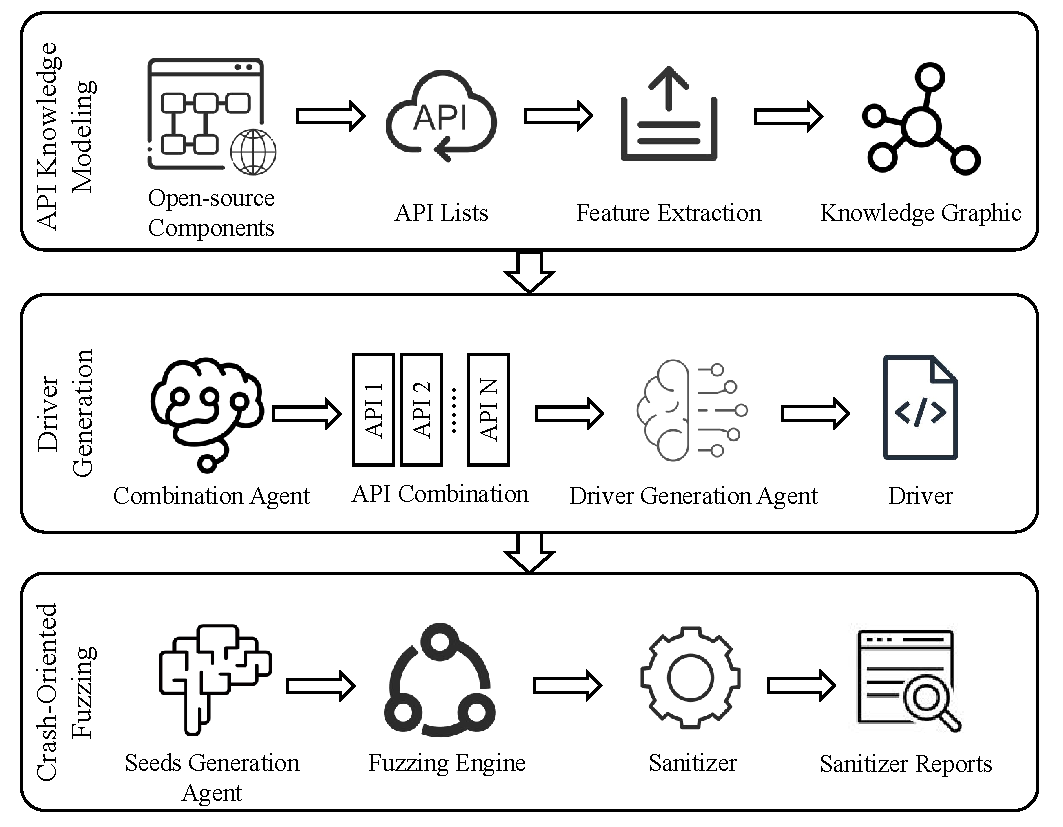
\includegraphics[width=0.75\linewidth]{figures/fig1.pdf}
\caption{Overview of the LLM-assisted fuzzing framework.}
\label{fig:fig1}
\end{figure}

\subsection{Challenges Statement}

Unlike conventional fuzzing, LLM-assisted fuzzing cannot assume that the generated driver is a trusted harness \citep{ref12,ref13}. A reported crash may result from the target component, the generated driver, or their interaction under a mutated input. Consequently, the crash report alone may not provide sufficient evidence for reliable post-fuzzing analysis. This setting raises three challenges: false-alert judgment, crash localization, and efficiency.

\textbf{False-alert judgment.} An LLM-generated driver may violate implicit API contracts by omitting required initialization, constructing inconsistent object states, or passing invalid argument combinations. Such misuse can trigger a failure while execution is inside the target component, causing the sanitizer stack trace to contain component frames even when the underlying fault originates from the driver. The presence of a component frame therefore does not by itself establish target-component attribution. Distinguishing driver-induced failures from target-component-originated crashes is difficult because a raw report records where the failure becomes observable, but does not explicitly identify which side violated the required execution contract.

\textbf{Efficiency.} LLM-assisted fuzzing repeatedly mutates related inputs, so many crashing inputs may exercise the same underlying failure pattern. Different generated drivers may also reach that failure pattern through distinct API combinations or call paths. These executions can produce reports that differ in addresses, stack depth, or intermediate frames despite sharing one root cause \citep{ref21,ref22,ref25}. Treating every report as an independent case leads to repeated inspection and redundant LLM submissions, making crash adjudication increasingly expensive as the number of generated drivers and crashing inputs grows.

\textbf{Crash localization.} Existing prompt-based analysis commonly reasons over raw crash reports without explicitly localizing the failure across the generated driver and the target component. Because a driver-constructed invalid state may become observable only after entering component code, the visible crash frame can be mistaken for evidence that the open-source supply-chain component caused the failure. Localization information is therefore necessary not only to identify a suspicious statement, but also to determine where the faulty state originates and how it reaches the crash site \citep{ref14,ref15,ref20,ref23}. However, existing localization evidence is dominated by static code context, while runtime context is not systematically incorporated into driver/component attribution. Static code context cannot expose the concrete values, pointer states, or object states involved in the failing execution, leaving the propagation of the faulty state incomplete and crash attribution uncertain.


\section{Approach}
\label{sec:approach}

\subsection{CrashSage Design Overview}
\label{subsec:problem-overview}

In this section, we present the system design of CrashSage, an evidence-guided crash-adjudication framework for LLM-assisted fuzzing. CrashSage is designed to improve post-fuzzing crash adjudication when automatically generated fuzz drivers cannot be treated as trusted harnesses. Its primary objective is to prepare structured evidence that supports attribution-oriented localization, remove repeated crash instances, and retain auditable inputs before final LLM reasoning. Through this pipeline, CrashSage supports false-alert judgment, crash localization, and efficient analysis of repeatedly triggered crashes.

Figure~\ref{fig:three-mechanism-design} illustrates the workflow of CrashSage and aligns the three challenges with the corresponding processing stages. Initially, \emph{rule-guided crash attribution} addresses false-alert judgment by distinguishing noise and likely driver-induced crashes from cases that require further target-component analysis. It normalizes crash reports and applies rule-based preliminary screening over sanitizer signals and stack-frame roles, producing filtered normalized crash reports for the following stages. Next, \emph{representative selection} addresses efficiency by avoiding repeated analysis of crashes that follow the same underlying failure pattern. It constructs exact and stack signatures from the normalized sanitizer evidence, verifies signature matches, maps repeated crashes to an existing representative, and retains unmatched crashes in the selected crash set. CrashSage then performs \emph{crash-context reconstruction} to enrich these selected representatives with static code context and replay-consistent runtime context, helping determine where an invalid state originates and how it propagates to the visible crash site. Finally, \emph{LLM analysis} completes the semantic diagnosis by combining each representative crash's normalized crash report, triage label, and reconstructed context to determine its type, cause, location, triggering condition, and severity.


\begin{figure}[H]
\centering
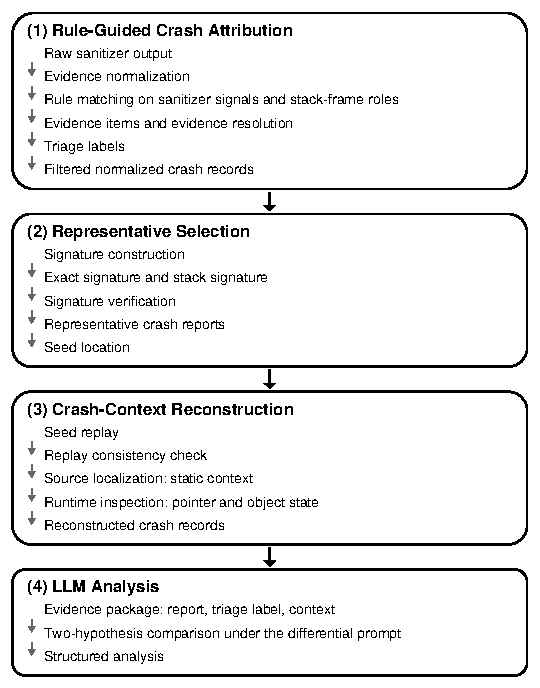
\includegraphics[width=0.75\linewidth]{figures/fig2.pdf}
\caption{Multi-stage crash-adjudication pipeline combining rule-guided crash attribution, representative selection, crash-context reconstruction, and LLM analysis.}
\label{fig:three-mechanism-design}
\end{figure}

\subsection{Rule-Guided Crash Attribution}
\label{subsec:rule-guided-attribution}

Rule-guided crash attribution is the first stage of CrashSage and addresses the false-alert judgment challenge.
It consists of sanitizer evidence normalization and rule-based preliminary screening.
The former converts raw sanitizer output into a normalized crash report, while the latter assigns a triage label that determines whether the crash is filtered.

\subsubsection{Sanitizer Evidence Normalization}
Crash reports contain substantial redundant information that is not directly useful for subsequent crash adjudication. 
CrashSage normalizes each raw crash report into a normalized crash report that retains the information required by subsequent stages.
Its fields fall into the six categories summarized below and in Table~\ref{tab:sanitizer-normalized-fields}.

\begin{itemize}
    \item \textbf{Failure identity} describes the crash report type and its failure category.
    \item \textbf{Crash-site metadata} records the immediate low-level crash information, such as the failing address or access behavior, when it is available.
    \item \textbf{Severity and dedup cues} provide sanitizer- or fuzzer-generated hints that help prioritize and compare crash reports.
    \item \textbf{Structured stack trace} converts the raw call stack into ordered frames for later role modeling.
    \item \textbf{Project anchor} identifies the first visible connection between the crash trace and the target-component source code.
    \item \textbf{Reproduction and status hints} preserve crash-input clues and special execution states that may affect filtering or replay.
\end{itemize}

\begin{table}[t]
\caption{Key field groups in the normalized crash report}
\label{tab:sanitizer-normalized-fields}
\centering
\compacttable
\setlength{\tabcolsep}{4.0pt}
\renewcommand{\arraystretch}{1.10}
\begin{tabular*}{\linewidth}{@{\extracolsep{\fill}}ll}
\toprule
\textbf{Field Group} & \textbf{Representative Extracted Fields} \\
\midrule
Failure identity & \texttt{sanitizer\_type}, \texttt{bug\_type}, \texttt{summary} \\
Crash-site metadata & \texttt{crash\_address}, \texttt{pc}, \texttt{access\_type} \\
Severity and dedup cues & \texttt{scariness\_score}, \texttt{scariness\_desc}, \texttt{dedup\_token} \\
Structured stack trace & ordered \texttt{frames} with function, file, line, and address \\
Project anchor & \texttt{first\_in\_project\_frame}, \texttt{first\_in\_project\_function} \\
Reproduction and status hints & \texttt{artifact\_path\_hint}, \texttt{base\_unit\_hash}, special-condition flags \\
\botrule
\end{tabular*}
\end{table}

\subsubsection{Rule-Based Preliminary Screening}
Screening begins by matching the function name, file path, and position of each frame in the \texttt{structured stack trace} against predefined project, driver, and runtime patterns.
Frames without sufficient matching evidence remain \emph{unclassified}.
Table~\ref{tab:stack-frame-roles} summarizes these roles.

\begin{table}[t]
\caption{Stack-frame role classification used by CrashSage}
\label{tab:stack-frame-roles}
\centering
\scriptsize
\setlength{\tabcolsep}{4.0pt}
\renewcommand{\arraystretch}{1.10}
\begin{tabular*}{\linewidth}{@{\extracolsep{\fill}}ll}
\toprule
\textbf{Role} & \textbf{Meaning} \\
\midrule
project & Stack frames in the target-component source code. \\
driver & Stack frames related to the fuzz driver. \\
runtime & Runtime-library frames, including libFuzzer, sanitizers, LLVM runtime, libc, etc. \\
unclassified & Frames that cannot be classified reliably but are not obvious runtime frames. \\
\botrule
\end{tabular*}
\end{table}

Frame ownership alone is not sufficient for false-alert judgment.
A crash trace can involve target-component frames, generated-driver frames, and runtime frames at the same time, while the frame where the sanitizer reports the failure may not be the frame that best explains the origin of the crash.
CrashSage therefore applies a set of deterministic rules over the ownership and position of stack frames to infer whether the crash is more consistent with noise, a driver-induced failure, or a target-component crash.

Before listing the rules, we define the following notations.
Let \(S=\langle f_1,\ldots,f_n\rangle\) denote the structured stack trace, ordered from the top crashing frame to lower caller frames.
Let \(F_P\), \(F_D\), and \(F_N\) denote the sets of project frames, driver frames, and non-runtime frames, respectively, where \(F_N=F_P\cup F_D\cup F_U\) and \(F_U\) is the set of unclassified frames.
CrashSage computes the driver-frame ratio
\begin{equation}
R_D=\frac{|F_D|}{\max(|F_N|,1)} ,
\end{equation}
corresponding to \texttt{Driver\_Frame\_Ratio}.
Runtime frames are excluded from this ratio because they mainly reflect sanitizer and libFuzzer control flow.
Let \(h_D\) denote the top-stack depth inspected for driver evidence, \(\theta_D\) the driver-frame-ratio threshold, \(m_P\) the maximum number of project frames treated as shallow project involvement, and \(\theta_S\) the sanitizer-severity threshold.

CrashSage sets these parameters through an evidence-boundary design strategy that maps each value to an interpretable stack or sanitizer signal.
The parameter \(h_D\) defines the near-crash stack region used for driver-evidence inspection, \(\theta_D\) defines the driver-dominance level in the attribution-relevant non-runtime stack, \(m_P\) defines the amount of project-code involvement treated as shallow API-boundary execution, and \(\theta_S\) defines the sanitizer-severity level used to retain project-frame SEGV/null-dereference reports.

For \(h_D\), CrashSage sets \(h_D=3\) because a three-frame window corresponds to the crash frame, the direct caller, and the caller that usually reflects the immediate driver-side invocation context.
This value keeps the check centered on the local failure path where argument construction, API invocation, and first observable faulty use are most directly represented.
For \(\theta_D\), CrashSage sets \(\theta_D=0.8\), using a four-fifths majority as the driver-dominance criterion over non-runtime frames.
This value requires driver evidence to occupy a clearly dominant share of the attribution-relevant stack before assigning \texttt{likely\_driver\_bug}, making the label depend on stack-level concentration rather than an isolated driver frame.
For \(m_P\), CrashSage sets \(m_P=2\) because shallow API-boundary execution often includes the target entry function and one adjacent helper, initialization, creation, setup, or parsing frame.
This value captures brief project-code contact during driver-constructed calls while distinguishing it from deeper target-component execution paths.
For \(\theta_S\), CrashSage sets \(\theta_S=10\) as the high-severity sanitizer threshold for SEGV/null-dereference reports.
This value retains reports when the sanitizer signal indicates severe invalid memory access and the stack simultaneously provides project-frame evidence for target-component analysis.

These values are fixed before evaluating the crash reports, providing a stable and reproducible configuration for the rule-guided attribution stage.

The remaining rule signals also come from the normalized crash report.
Timeout, \texttt{ALARM}, out-of-memory, LSan-only, and deadly-signal flags are extracted from sanitizer or libFuzzer status lines, while \texttt{SCARINESS} comes from the sanitizer severity line.
Table~\ref{tab:triage-rule-groups} lists the 13 rules and their output labels.

\begin{table}[t]
\caption{Rules used for crash attribution}
\label{tab:triage-rule-groups}
\centering
\compacttable
\setlength{\tabcolsep}{2.4pt}
\renewcommand{\arraystretch}{1.10}
\begin{tabularx}{\linewidth}{C{0.08\linewidth} C{0.08\linewidth} Y L{0.19\linewidth}}
\toprule
\textbf{Group} & \textbf{Rule} & \textbf{Deterministic Predicate} & \textbf{Output Label} \\
\midrule
NF & R1 & \(F_N=\emptyset \land \texttt{deadly\_signal}\) & \texttt{noise} \\
NF & R2 & Timeout or \texttt{ALARM} marker appears & \texttt{noise} \\
NF & R3 & Out-of-memory marker appears & \texttt{noise} \\
NF & R4 & LSan-only report without crashing execution & \texttt{noise} \\
\midrule
DQ & R5 & \(\texttt{use\_of\_uninitialized\_value}\) with a driver frame in the top-\(h_D\) stack frames & \texttt{likely\_driver\_bug} \\
DQ & R6 & \(R_D\ge \theta_D\) & \texttt{likely\_driver\_bug} \\
DQ & R7 & Project init/option/parse function appears near the driver boundary & \texttt{likely\_driver\_bug} \\
DQ & R8 & \(\texttt{stack\_buffer\_overflow}\) with the top frame in driver code & \texttt{likely\_driver\_bug} \\
DQ & R9 & \(F_N=F_D \land F_P=\emptyset\) & \texttt{likely\_driver\_bug} \\
DQ & R10 & \(|F_P|\le m_P\) and project function matches init/create patterns & \texttt{likely\_driver\_bug} \\
\midrule
TC & R11 & Memory-safety crash with at least one project frame & \texttt{target\_crash} \\
TC & R12 & SEGV/null-dereference with \(\texttt{SCARINESS}\ge \theta_S\) and project frame evidence & \texttt{target\_crash} \\
\midrule
LE & R13 & Assertion or abort originates in project code & \texttt{needs\_review} \\
\botrule
\end{tabularx}
\vspace{2pt}
{\raggedright\scriptsize \textit{Note.} NF: noise filtering; DQ: driver-quality detection; TC: target-component attribution indication; LE: logic-error indication. \(F_N\), \(F_D\), and \(F_P\) denote non-runtime, driver, and project frame sets, respectively.\par}
\end{table}

The rationale for each rule and its preliminary output label is described below.
These labels express the direction supported by the available evidence rather than a final vulnerability verdict.

\begin{itemize}
    \item \textbf{R1.} A \texttt{deadly\_signal} marker confirms abnormal termination, but the absence of non-runtime frames leaves no project or driver location for attribution. The report is therefore labeled \texttt{noise} because it provides no inspectable evidence for the subsequent analysis.
    \item \textbf{R2.} Timeout and \texttt{ALARM} markers indicate that execution exceeded its time limit, without providing sanitizer evidence for a memory-access crash. Such reports are labeled \texttt{noise} because they do not provide crash evidence for component attribution.
    \item \textbf{R3.} An out-of-memory marker records resource exhaustion, which may depend on allocation demand or execution limits and does not identify a specific faulty access. The rule therefore assigns \texttt{noise} rather than attributing the condition to either the driver or the target component.
    \item \textbf{R4.} An LSan-only report identifies unreleased allocations at process exit but contains no crashing instruction, signal, or abort. Because the rule-guided stage concerns the origin of crashes, this report is labeled \texttt{noise}.
    \item \textbf{R5.} An uninitialized-value report indicates that data was consumed before receiving a valid value. When driver frames occur within the top \(h_D\) frames, the first observable use is close to driver-side execution, so the available evidence supports \texttt{likely\_driver\_bug}.
    \item \textbf{R6.} After runtime frames are removed, \(R_D\ge \theta_D\) means that driver frames account for the specified dominant share of the attribution-relevant stack. Because the observable crash path is concentrated in the generated harness, the rule assigns \texttt{likely\_driver\_bug}.
    \item \textbf{R7.} Initialization, option-processing, and parsing functions near the driver boundary are commonly reached while the generated driver constructs objects and prepares API arguments. When project involvement remains at this boundary, the evidence favors invalid driver-side setup over target-component-originated execution, leading to \texttt{likely\_driver\_bug}.
    \item \textbf{R8.} For a stack-buffer overflow, the top frame identifies the function whose active stack object exceeds its boundary. If this frame belongs to the driver, the overflowing object is localized to driver-side execution, so the rule assigns \texttt{likely\_driver\_bug}.
    \item \textbf{R9.} If every non-runtime frame belongs to the driver and no project frame is present, the trace contains no observable evidence that execution reached target-component code. The crash is therefore labeled \texttt{likely\_driver\_bug}.
    \item \textbf{R10.} At most \(m_P\) project frames limited to initialization or creation functions indicate shallow component involvement during API setup rather than an internal target execution path. This pattern is treated as \texttt{likely\_driver\_bug} because the evidence primarily reflects how the generated driver configured the call.
    \item \textbf{R11.} A sanitizer-reported memory-safety crash with at least one project frame establishes that the erroneous execution reached target-component code. The rule labels it \texttt{target\_crash} so that it is retained as a target-component-attributed candidate for subsequent stages, rather than making the final attribution decision in the rule-guided stage.
    \item \textbf{R12.} A severe SEGV or null dereference indicates an invalid memory access, while the presence of project frames anchors that access in target-component execution. Their combination supports the preliminary label \texttt{target\_crash} and retains the crash for localization.
    \item \textbf{R13.} A project-origin assertion or abort identifies the component location that terminates execution, but the report alone cannot distinguish a driver violation of an API precondition from a violated internal invariant. The rule therefore assigns \texttt{needs\_review} rather than attributing the crash to either side.
\end{itemize}

Because the rules are evaluated independently, CrashSage resolves their evidence items in the order \texttt{noise}, \texttt{likely\_driver\_bug}, \texttt{target\_crash}, and \texttt{needs\_review}.
The first matched label in this order becomes the triage label; if no rule matches, the crash is assigned \texttt{needs\_review} by default.
This procedure removes reports without usable crash evidence and generated-driver crashes before retaining target-component-attributed candidates and ambiguous cases for further analysis.

Crashes labeled \texttt{noise} or \texttt{likely\_driver\_bug} are filtered, whereas those labeled \texttt{target\_crash} or \texttt{needs\_review} are kept as retained normalized crash reports for representative selection.
For a crash \(c\), let \(\mathcal{N}(c)\) denote its normalized crash report and \(y(c)\) denote its triage label.
The output of rule-guided crash attribution is the pair \(\langle\mathcal{N}(c),y(c)\rangle\), which serves as the input to the subsequent stage.


\subsection{Representative Selection}

Large-scale fuzzing often produces many crash instances that differ in inputs or generated drivers but follow the same underlying failure pattern.
Representative selection reduces this repeated analysis cost by comparing exact and stack signatures and forwarding only non-duplicate representatives to the later LLM stage.

Let \(\mathcal{C}=\{c_1,\ldots,c_n\}\) denote the set of crashes retained after rule-guided crash attribution.
For each crash \(c\), let \(S_c\) denote its structured stack trace following the definition of \(S\) in Section~\ref{subsec:rule-guided-attribution}, and let \(d(c)\) denote the sanitizer deduplication token.
Let \(b(c)\) denote the sanitizer bug type extracted from \(\mathcal{N}(c)\), and let \(\ell(c)\) denote the crash-site source location derived from the crash-site metadata or resolved frame location when available.
Let \(\bot\) denote an unavailable value.
The sequence \(s(c)\) is the ordered non-runtime key-frame subsequence derived from \(S_c\).
Runtime frames are excluded from \(s(c)\) because they usually describe sanitizer, libFuzzer, or libc control flow rather than the project-driver execution path.

\textbf{Exact signature.} The exact signature targets crashes with the same sanitizer-provided identity or the same resolved crash site.
CrashSage computes
\begin{equation}
\sigma_{\mathrm{exact}}(c)=
\begin{cases}
H(d(c)), & d(c)\neq \bot,\\
H\bigl(b(c),\ell(c),\mathrm{top}(s(c))\bigr), & d(c)=\bot \land \ell(c)\neq \bot \land |s(c)|>0,\\
\bot, & \text{otherwise},
\end{cases}
\end{equation}
where \(H(\cdot)\) is a stable hash function and \(\mathrm{top}(s(c))\) denotes the first frame in the non-runtime key-frame sequence.
The exact-signature match between two crashes is defined as
\begin{equation}
M_{\mathrm{exact}}(c_i,c_j)=
\mathbb{I}\bigl[
\sigma_{\mathrm{exact}}(c_i)\neq \bot
\land \sigma_{\mathrm{exact}}(c_i)=\sigma_{\mathrm{exact}}(c_j)
\bigr].
\end{equation}
Here, \(M_{\mathrm{exact}}(c_i,c_j)=1\) represents the strongest duplicate match.
The condition holds either because both crashes expose the same sanitizer deduplication token \(d(c)\), or because the normalized fields \(b(c)\), \(\ell(c)\), and \(\mathrm{top}(s(c))\) agree.
In the latter case, the two reports have the same sanitizer crash class, the same localized crash-site anchor such as file, line, and function, and the same first project/driver frame after runtime frames are removed.

\textbf{Stack signature.} The stack signature targets crashes whose crash-site anchors differ but whose project-driver call paths are identical.
Let \(p_k(c)\) denote the ordered sequence obtained by taking the first \(\min(k,|s(c)|)\) frames from \(s(c)\), preserving the original stack order from the top crashing frame to lower caller frames.
Here, \(k\) is a fixed prefix length used consistently for all crashes.
CrashSage builds a stack signature from this bounded prefix:
\begin{equation}
\sigma_{\mathrm{stack}}(c)=H\bigl(b(c),p_k(c)\bigr).
\end{equation}
The bug type is kept in the signature to avoid treating different sanitizer crash classes that happen to pass through similar functions as duplicates.
The bounded prefix of the non-runtime stack captures the driver-to-project execution path that reaches the crash.
The stack-signature match is defined as
\begin{equation}
M_{\mathrm{stack}}(c_i,c_j)=
\mathbb{I}\bigl[
\sigma_{\mathrm{stack}}(c_i)=\sigma_{\mathrm{stack}}(c_j)
\bigr].
\end{equation}
Here, \(M_{\mathrm{stack}}(c_i,c_j)=1\) represents a duplicate match based on the retained call path rather than on an identical crash-site anchor.
The equality of \(\sigma_{\mathrm{stack}}\) requires the same \(b(c)\) and the same bounded prefix \(p_k(c)\), where \(p_k(c)\) is built from the ordered non-runtime frames in \(s(c)\).
Thus, the two crashes are treated as duplicates when their normalized stack evidence shows the same sanitizer crash class and the same leading project/driver frame sequence, even if the reported line number, resolved crash location, or exact sanitizer token is unavailable or slightly different.

CrashSage evaluates the two match predicates in the order of exact and stack matching, which corresponds to signature verification in Figure~\ref{fig:three-mechanism-design}.
For a pair of crashes, stack matching is evaluated only when exact matching does not produce a match.
The resulting duplicate decision is
\begin{equation}
M(c_i,c_j)=
M_{\mathrm{exact}}(c_i,c_j)
\lor M_{\mathrm{stack}}(c_i,c_j).
\end{equation}

CrashSage processes the retained crashes in discovery order and compares each crash with the representatives selected so far.
A matched crash is linked to the corresponding representative, whereas an unmatched crash becomes a new representative.
Algorithm~\ref{alg:representative-selection} summarizes this procedure.

\begin{algorithm}[t]
\caption{Representative Selection}
\label{alg:representative-selection}
\begin{algorithmic}
\Require retained crashes \(\mathcal{C}=\langle c_1,\ldots,c_n\rangle\) in discovery order
\Ensure selected crash set \(\mathcal{R}\) and duplicate mapping \(\mathcal{L}\)
\State \(\mathcal{R}\gets\varnothing\), \(\mathcal{L}\gets\varnothing\)
\For{\(c_i\in\mathcal{C}\)}
    \State \(r^\ast\gets\bot\)
    \For{\(r\in\mathcal{R}\)}
        \If{\(M(c_i,r)=1\)}
            \State \(r^\ast\gets r\)
            \State \textbf{break}
        \EndIf
    \EndFor
    \If{\(r^\ast\neq\bot\)}
        \State \(\mathcal{L}\gets\mathcal{L}\cup\{(c_i,r^\ast)\}\)
    \Else
        \State \(\mathcal{R}\gets\mathcal{R}\cup\{c_i\}\)
    \EndIf
\EndFor
\State \Return \((\mathcal{R},\mathcal{L})\)
\end{algorithmic}
\end{algorithm}

The primary output of representative selection is the selected crash set \(\mathcal{R}\).
The accompanying mapping \(\mathcal{L}\) records each duplicate--representative pair \((c_i,r)\), indicating that \(c_i\) matches and reuses the analysis result of representative \(r\).


\subsection{Crash-Context Reconstruction}

After representative selection, the selected crash representatives still require relevant localization evidence to refine the attribution.
A component frame identifies where a failure becomes visible, but it does not establish whether the faulty state originates in the generated driver or the target component.
Crash-context reconstruction addresses this gap through static code context reconstruction and runtime context reconstruction.
Static code context reconstruction maps the driver-to-component call path to source code, while runtime context reconstruction recovers the execution state needed to explain how the failure propagates along that path.
Together, they turn an isolated sanitizer crash label into attribution-oriented execution evidence for LLM adjudication of the selected representatives.

\subsubsection{Static Code Context Reconstruction}
Static code context reconstruction localizes selected project and driver frames in a representative crash report to source files and extracts the surrounding source-code context.
CrashSage first maps each selected frame to a local file, function, and line number using the reported source coordinates.
Based on these locations, it extracts bounded code windows around the crash-site frame and relevant call-chain frames, preserving the local statements before and after each key frame.
These code windows provide source-level evidence for inspecting the crashing operation and tracing how the fuzz input moves from the generated driver into the target API and toward the crash site.
However, static code context alone cannot determine the concrete values and object states present in the failing execution.

\subsubsection{Runtime Context Reconstruction}
Runtime context reconstruction complements static code context reconstruction by recovering execution-state evidence that static code alone cannot provide, including variable values, pointer states, and memory-related conditions at the crash point.
This evidence helps determine whether an invalid state is constructed by the driver and propagated into component code or produced within the component itself.
CrashSage uses \texttt{artifact\_path\_hint} or \texttt{base\_unit\_hash} in the normalized crash report to locate the triggering seed and stage an isolated copy for replay.

Replaying the seed is necessary to observe the execution state at the crash point.
However, environmental differences, timing-dependent behavior, uninitialized state, or external resources may cause the same seed to produce a different crash.
CrashSage therefore parses the replayed crash report into a replay-produced normalized crash record and verifies its consistency before collecting runtime context.
To bind the replay result to the representative crash, CrashSage builds a replay key
\begin{equation}
\kappa(c)=\langle b(c), \ell(c), s(c) \rangle ,
\end{equation}
where \(b(c)\) corresponds to the \texttt{bug\_type} field of crash report \(c\), \(\ell(c)\) denotes the crash-site source location derived from the crash-site metadata or resolved frame location when available, and \(s(c)\) denotes the ordered non-runtime key-frame sequence derived from the structured stack trace \(S\).
Let \(c_0\) denote the original normalized crash report and \(c_r\) denote the replay-produced crash record.
CrashSage regards their replay keys as compatible, denoted by \(\kappa(c_r)\simeq\kappa(c_0)\), when
\begin{equation}
b(c_r)=b(c_0) \land s(c_r)=s(c_0) \land
\bigl(\ell(c_0)=\bot \lor \ell(c_r)=\ell(c_0)\bigr),
\end{equation}
where \(\bot\) denotes an unavailable value in the corresponding field.
Only a replay satisfying this condition is treated as consistent with the representative crash and used for runtime inspection.

For a replay-consistent crash, CrashSage invokes GDB as the runtime inspection tool.
The bounded GDB run records the reproduced backtrace and crash frame, together with selected registers, function arguments, and local variables from the frames nearest to the crash site.
These fields can help reveal state that static code context cannot provide, such as whether a pointer is null, whether a size variable is inconsistent with a buffer, or whether an object has an invalid state before the crashing operation.

Algorithm~\ref{alg:runtime-context} summarizes this reproduction-gated runtime context reconstruction procedure.

\begin{algorithm}[t]
\caption{Runtime Context Reconstruction}
\label{alg:runtime-context}
\begin{algorithmic}
\Require normalized crash report \(c_0\), static code context \(C_{\mathrm{static}}\), fuzz target binary \(B\), corpus or artifact directory \(D\)
\Ensure reconstructed context \(C_{\mathrm{recon}}(c_0)=(C_{\mathrm{static}}, C_{\mathrm{runtime}}, \rho)\)
\State \(u \gets \Call{LocateSeed}{c_0.\texttt{artifact\_path\_hint}, c_0.\texttt{base\_unit\_hash}, D}\)
\If{\(u\) is unavailable}
    \State \Return \((C_{\mathrm{static}}, \bot, \textsc{SeedUnavailable})\)
\EndIf
\State \(u_s \gets \Call{StageSeed}{u}\)
\State \(c_r \gets \Call{ReplayAndParse}{u_s, B}\)
\If{\(c_r\) is unavailable}
    \State \Return \((C_{\mathrm{static}}, \bot, \textsc{ReplayFailed})\)
\EndIf
\If{\(\kappa(c_r)\not\simeq\kappa(c_0)\)}
    \State \Return \((C_{\mathrm{static}}, \bot, \textsc{CrashMismatch})\)
\EndIf
\State \(C_{\mathrm{runtime}} \gets \Call{CollectDebugContext}{u_s, B}\)
\If{\(C_{\mathrm{runtime}}\) is unavailable}
    \State \Return \((C_{\mathrm{static}}, \bot, \textsc{RuntimeContextUnavailable})\)
\EndIf
\State \(\rho \gets \textsc{RuntimeContextAvailable}\)
\State \Return \((C_{\mathrm{static}}, C_{\mathrm{runtime}}, \rho)\)
\end{algorithmic}
\end{algorithm}

\begin{table}[t]
\caption{Evidence groups produced by crash-context reconstruction}
\label{tab:reconstruction-output-fields}
\centering
\compacttable
\setlength{\tabcolsep}{3.8pt}
\renewcommand{\arraystretch}{1.10}
\begin{tabularx}{\linewidth}{L{0.16\linewidth} L{0.22\linewidth} L{0.31\linewidth} Y}
\toprule
\textbf{Context Type} & \textbf{Evidence Group} & \textbf{Representative Fields} & \textbf{Concrete Role} \\
\midrule
\multirow{2}{=}{Static code context}
& Crash-site anchor
& \texttt{crash\_file}, \texttt{crash\_line}, \texttt{crash\_function}, \texttt{crash\_code\_snippet}
& Anchors the visible crash site without treating it as the fault origin. \\
\cmidrule(l){2-4}
& Call-chain source context
& \texttt{call\_chain\_context}, \texttt{frame\_type}, \texttt{code\_snippet}
& Preserves bounded project/driver frame context for attribution. \\
\midrule
\multirow{3}{=}{Runtime context}
& Seed recovery and isolation metadata
& \texttt{seed\_locate}, \texttt{seed\_copy}, \texttt{seed\_paths.seed}
& Records how the triggering artifact is recovered and staged. \\
\cmidrule(l){2-4}
& Replay consistency evidence
& \texttt{repro.runs}, \texttt{signature}, \texttt{same\_signature}, \texttt{repro\_rate}
& Audits whether replay matches the representative crash. \\
\cmidrule(l){2-4}
& Runtime execution context
& \texttt{reproduced}, \texttt{backtrace\_text}, \texttt{registers}, \texttt{crash\_frame}, \texttt{call\_stack}
& Supplies runtime state for tracing fault propagation and refining attribution. \\
\botrule
\end{tabularx}
\end{table}
\FloatBarrier

\textsc{LocateSeed}, \textsc{StageSeed}, \textsc{ReplayAndParse}, and \textsc{CollectDebugContext} correspond to seed recovery, isolated replay preparation, replay-output parsing, and GDB-based bounded runtime-state collection, respectively.
For each representative crash \(c\in\mathcal{R}\), the output \(C_{\mathrm{recon}}(c)\) contains static code context, optional runtime context, and a status \(\rho\) indicating the outcome of seed recovery, replay matching, and GDB collection.
If runtime evidence is unavailable, \(C_{\mathrm{runtime}}=\bot\), and the static context remains available to subsequent stages.
Table~\ref{tab:reconstruction-output-fields} organizes the evidence groups by context type and summarizes their representative fields and roles in subsequent analysis.

For each representative crash \(c\in\mathcal{R}\), crash-context reconstruction outputs \(C_{\mathrm{recon}}(c)\). After this stage, the evidence package consumed by the final LLM analysis is defined as
\begin{equation}
\mathbf{x}(c)=
\left\langle
\mathcal{N}(c),\,y(c),\,C_{\mathrm{recon}}(c)
\right\rangle .
\end{equation}
This package combines the normalized crash report and triage label from rule-guided attribution with the reconstructed context produced in this stage.


\subsection{LLM Analysis}
\label{subsec:llm-analysis}

Given the evidence package \(\mathbf{x}(c)\), CrashSage invokes the LLM only for representative crashes \(c\in\mathcal{R}\). The LLM produces a structured diagnosis
through schema-guided, evidence-guided prompting rather than direct classification over raw sanitizer text.
Table~\ref{tab:llm-prompt-design} summarizes the prompt design sent to the LLM for each representative crash.

\begin{table}[t]
\caption{Prompt design for LLM analysis}
\label{tab:llm-prompt-design}
\centering
\compacttable
\setlength{\tabcolsep}{4pt}
\renewcommand{\arraystretch}{1.10}
\begin{tabularx}{\linewidth}{L{0.22\linewidth} Y}
\toprule
\textbf{Prompt Part} & \textbf{Prompt Design} \\
\midrule
System role
& Act as a crash-adjudication assistant and distinguish the visible crash site from the origin of the faulty state. \\
\midrule
Attribution rule
& Do not assign target-component attribution unless target-component evidence is stronger than the driver-misuse hypothesis. \\
\midrule
Input evidence
& Use the triage summary, matched rules, frame-role evidence, normalized sanitizer fields, static context, runtime context, and duplicate-cluster metadata. \\
\midrule
Label-conditioned task
& For \texttt{target\_crash}, verify the target-component root-cause hypothesis. For \texttt{needs\_review}, compare driver-defect and target-component-defect hypotheses. \\
\midrule
Examples
& No few-shot examples are used. \\
\midrule
Output schema
& Return \texttt{target\_attribution}, \texttt{root\_cause\_type}, \texttt{root\_cause\_location}, \texttt{triggering\_condition}, \texttt{severity}, \texttt{fix\_suggestion}, and \texttt{evidence\_rationale}. \\
\midrule
Decoding and retry
& Use \texttt{temperature=0}; retry once with a schema-repair instruction if the response is unparsable or incomplete. \\
\botrule
\end{tabularx}
\end{table}

For each representative, CrashSage serializes \(\mathbf{x}(c)\) into this staged prompt.
Runtime evidence is injected when replay succeeds; otherwise, the prompt records the unavailable runtime status instead of hiding the missing evidence.

The analysis task is conditioned on the triage label.
For \texttt{target\_crash}, the prompt asks the model to verify whether the target-component root-cause hypothesis is supported by the reconstructed evidence.
For \texttt{needs\_review}, the prompt asks the model to compare a driver-defect hypothesis against a target-component-defect hypothesis and to identify which side is better supported.
This differential framing keeps driver misuse in scope and reduces the tendency to over-attribute a component-visible crash to the target component.

The model output is required to follow a structured schema with the fields \texttt{target\_attribution}, \texttt{root\_cause\_type}, \texttt{root\_cause\_location}, \texttt{triggering\_condition}, \texttt{severity}, \texttt{fix\_suggestion}, and \texttt{evidence\_rationale}.
These fields correspond to the following diagnosis tuple:
\begin{equation}
\mathbf{z}(c)=
\left\langle
a(c),\,\tau(c),\,\lambda(c),\,\gamma(c),\,\nu(c),\,\phi(c)
\right\rangle ,
\end{equation}
where \(a(c)\) denotes the final target-component attribution judgment, \(\tau(c)\) denotes the root-cause type, \(\lambda(c)\) denotes the root-cause location, \(\gamma(c)\) denotes the triggering condition, \(\nu(c)\) denotes the severity, and \(\phi(c)\) denotes the repair suggestion.
The \texttt{evidence\_rationale} field records the short evidence chain supporting these schema fields and remains part of the report metadata.
If the second schema-repair attempt still fails validation, the deterministic evidence package is preserved and the LLM diagnosis is marked incomplete.
The final structured report is defined as
\begin{equation}
\mathbf{r}(c)=
\left\langle
\mathbf{x}(c),\,\mathbf{z}(c)
\right\rangle .
\end{equation}
This report preserves the deterministic evidence prepared by CrashSage together with the LLM-generated semantic diagnosis.



\section{Evaluation}
\label{sec:evaluation}

To evaluate the performance of CrashSage, we defined three research questions:

\begin{itemize}
    \item \textbf{RQ1: False-alert judgment}: How effectively does rule-guided crash attribution distinguish driver-induced crashes from target-component-attributed crashes?
    \item \textbf{RQ2: Efficiency}: How much redundant analysis does representative selection remove, and what latency do the major pipeline operations introduce?
    \item \textbf{RQ3: Crash localization}: How does crash-context reconstruction improve crash attribution and root-cause localization?
\end{itemize}

\subsection{Experimental Setup}

CrashSage is implemented in Python and uses Qwen3-Coder-Plus, accessed through a cloud API, as the LLM backend. All experiments are conducted on a machine running Ubuntu 22.04 and equipped with an AMD Ryzen 5 5600G with Radeon Graphics processor.

We select four open-source supply-chain components commonly used in ICV software stacks: c-ares, cJSON, libpcap, and zlib. Table~\ref{tab:subjects} summarizes their functions, API scales, and representative deployment roles.

\begin{table}[ht]
\caption{Open-source supply-chain components used in the evaluation}
\label{tab:subjects}
\centering
\compacttable
\scriptsize
\setlength{\tabcolsep}{3pt}
\renewcommand{\arraystretch}{1.18}
\begin{tabularx}{\linewidth}{L{0.14\linewidth} L{0.28\linewidth} C{0.07\linewidth} C{0.10\linewidth} Y}
\toprule
\textbf{Component} & \textbf{Function} & \textbf{APIs} & \makecell{\textbf{Crash}\\\textbf{Reports}} & \textbf{Deployment Role} \\
\midrule
c-ares & Asynchronous DNS resolution & 26 & 45 & Gateway DNS \\
cJSON & JSON parsing and generation & 59 & 30 & Config/telemetry parsing \\
libpcap & Packet capture and filtering & 29 & 41 & Network monitoring \\
zlib & Compression and decompression & 28 & 7 & OTA/log compression \\
\textbf{Combined} & -- & \textbf{142} & \textbf{123} & -- \\
\botrule
\end{tabularx}
\vspace{2pt}
\end{table}

We generate the crash reports following the fuzz-driver generation and fuzzing workflow of CKGFuzzer \citep{ref12}. The generated drivers are compiled and executed by libFuzzer with ASan+UBSan instrumentation in Docker containers based on the OSS-Fuzz base-runner image. Each driver is fuzzed for 1 hour, and the resulting sanitizer outputs are collected as crash reports, yielding 123 reports in total.

To evaluate the contributions of rule-guided crash attribution, representative selection, and crash-context reconstruction, we construct four controlled variants:
\begin{itemize}
    \item \textbf{V0} uses CKGFuzzer's original crash-cause classification module, which performs prompt-based classification using the raw crash report, fuzz-driver source, target-component source, and LLM-extracted error patterns.
    \item \textbf{V1} adds rule-guided crash attribution to V0.
    \item \textbf{V2} combines rule-guided crash attribution and representative selection without crash-context reconstruction.
    \item \textbf{V3 (CrashSage)} integrates rule-guided crash attribution, representative selection, and crash-context reconstruction into the complete pipeline.
\end{itemize}
Representative selection and crash-context reconstruction are evaluated after rule-guided crash attribution. Representative selection determines which retained reports are submitted to LLM analysis, and crash-context reconstruction supplies additional evidence for the selected representatives. We therefore do not construct variants that apply either module independently without rule-guided crash attribution.

For metric reporting, we use four external LLM adjudicators: GPT-5.5, Opus 4.8, Kimi-2.7-Coder, and Qwen3.7-Max. Each adjudicator receives the same crash evidence package and returns a binary target-component attribution judgment. We report precision, recall, and F1 separately under these adjudicators and use them for conservative relative comparison among variants. These adjudicators provide a consistent comparison protocol across variants, and the reported metrics are interpreted as relative attribution outcomes under the same evidence and adjudication setting. We also inspected representative reports after CrashSage processing and found that the recorded evidence was generally consistent with the corresponding filtering or retention decisions.

\FloatBarrier
\subsection{Evaluation of Rule-Guided Crash Attribution}

To evaluate rule-guided crash attribution, we compare V1 with V0 on the same 123 crash reports. Reports labeled \texttt{target\_crash} or \texttt{needs\_review} are forwarded to subsequent analysis after reports labeled \texttt{noise} or \texttt{likely\_driver\_bug} are filtered. We use precision to measure the proportion of predicted target-component-attributed crashes that are supported by the external adjudicator, recall to measure the proportion of adjudicator-supported target-component-attributed crashes identified by the variant, and F1 to reflect their overall balance. Because the external adjudicators require specific evidence for target-component attribution, these metrics provide a conservative basis for comparing variants.

\begin{figure}[H]
\centering
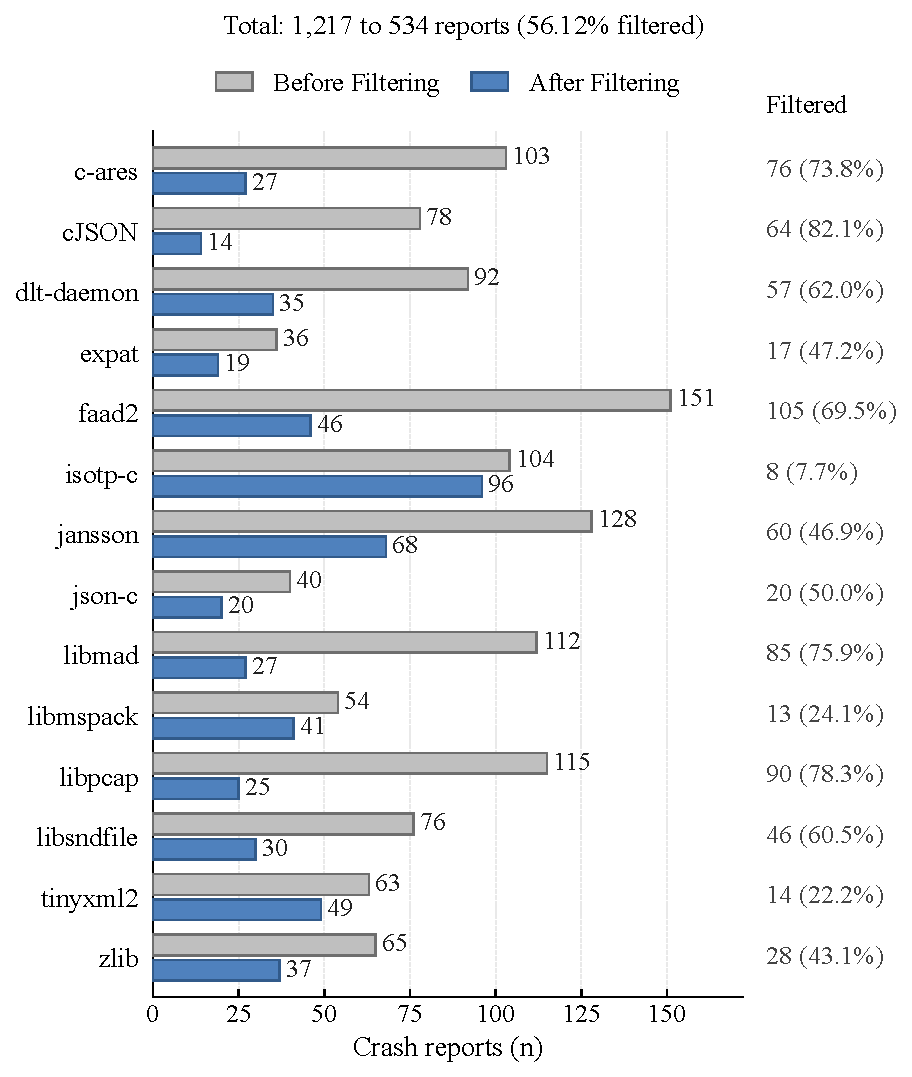
\includegraphics[width=0.75\linewidth]{figures/fig3.pdf}
\caption{Reduction in crash reports after rule-guided crash attribution.}
\label{fig:rule-guided-filtering}
\end{figure}

\begin{table}[ht]
\caption{Effect of rule-guided crash attribution under different external adjudicators.}
\label{tab:ablation-v0-v1}
\centering
\scriptsize
\setlength{\tabcolsep}{3.2pt}
\renewcommand{\arraystretch}{1.12}
\begin{tabular*}{\linewidth}{@{\extracolsep{\fill}}lcc|cc|cc}
\toprule
\textbf{External Adjudicator} & \textbf{V0 P} & \textbf{V1 P} & \textbf{V0 R} & \textbf{V1 R} & \textbf{V0 F1} & \textbf{V1 F1} \\
\midrule
GPT-5.5 & 0.000 & 0.042 & 0.000 & 1.000 & 0.000 & 0.080 \\
Opus 4.8 & 0.029 & 0.042 & 0.333 & 0.333 & 0.053 & 0.074 \\
Kimi-2.7-Coder & 0.029 & 0.125 & 0.100 & 0.300 & 0.044 & 0.176 \\
Qwen3.7-Max & 0.029 & 0.083 & 0.333 & 0.667 & 0.053 & 0.148 \\
\botrule
\end{tabular*}
\end{table}

The experimental results are shown in Figure~\ref{fig:rule-guided-filtering} and Table~\ref{tab:ablation-v0-v1}. Rule-guided crash attribution reduces the number of retained reports from 123 to 95 by filtering 28 reports before subsequent analysis. Across the four adjudicators, V1 improves F1 over V0 in every case, with F1 changing from 0.000--0.053 for V0 to 0.074--0.176 for V1. The low absolute F1 values reflect the conservative attribution criterion and the noisy crash reports produced by untrusted generated drivers, so the comparison emphasizes the consistent relative improvement from V0 to V1.

This result is mainly attributable to the reports removed by rule-guided crash attribution. Reports with insufficient crash evidence or evidence more consistent with driver-induced failures can introduce misleading information into subsequent analysis. Filtering these reports reduces driver-side cases entering later LLM analysis while preserving the target-component-attributed candidates that warrant further analysis. In response to RQ1, rule-guided crash attribution distinguishes driver-induced crashes from target-component-attributed crashes by filtering 28 reports while improving the attribution metrics under the four external adjudicators.

\FloatBarrier
\subsection{Evaluation of Representative Selection}

To evaluate the efficiency of representative selection, we compare V0 and V3. We first examine the time required by the major CrashSage modules and then distinguish the reduction caused by rule-guided filtering from the reduction caused by representative selection over the retained reports.

\begin{table}[ht]
\caption{Latency of the major modules in CrashSage.}
\label{tab:stage-latency}
\centering
\compacttable
\setlength{\tabcolsep}{4pt}
\begin{tabular*}{\linewidth}{@{\extracolsep{\fill}}lc}
\toprule
\textbf{Module} & \textbf{Typical Time per Report} \\
\midrule
Rule-guided crash attribution & \textless{} 10 ms \\
Crash-context reconstruction & \textasciitilde{}2,000--15,000 ms \\
Representative selection & \textless{} 5 ms \\
LLM analysis & \textasciitilde{}30,000--60,000 ms \\
\botrule
\end{tabular*}
\end{table}

As shown in Table~\ref{tab:stage-latency}, rule-guided crash attribution and representative selection each require less than 10 ms per report. In contrast, crash-context reconstruction requires approximately 2--15 s because it replays the crashing input and collects runtime state, while LLM analysis requires approximately 30--60 s because it depends on remote model inference. These two modules therefore account for most of the analysis time. The cost of crash-context reconstruction is partly reduced by rule-guided crash attribution, which filters 28 of the 123 crash reports before reconstruction is performed.

\begin{figure}[H]
\centering
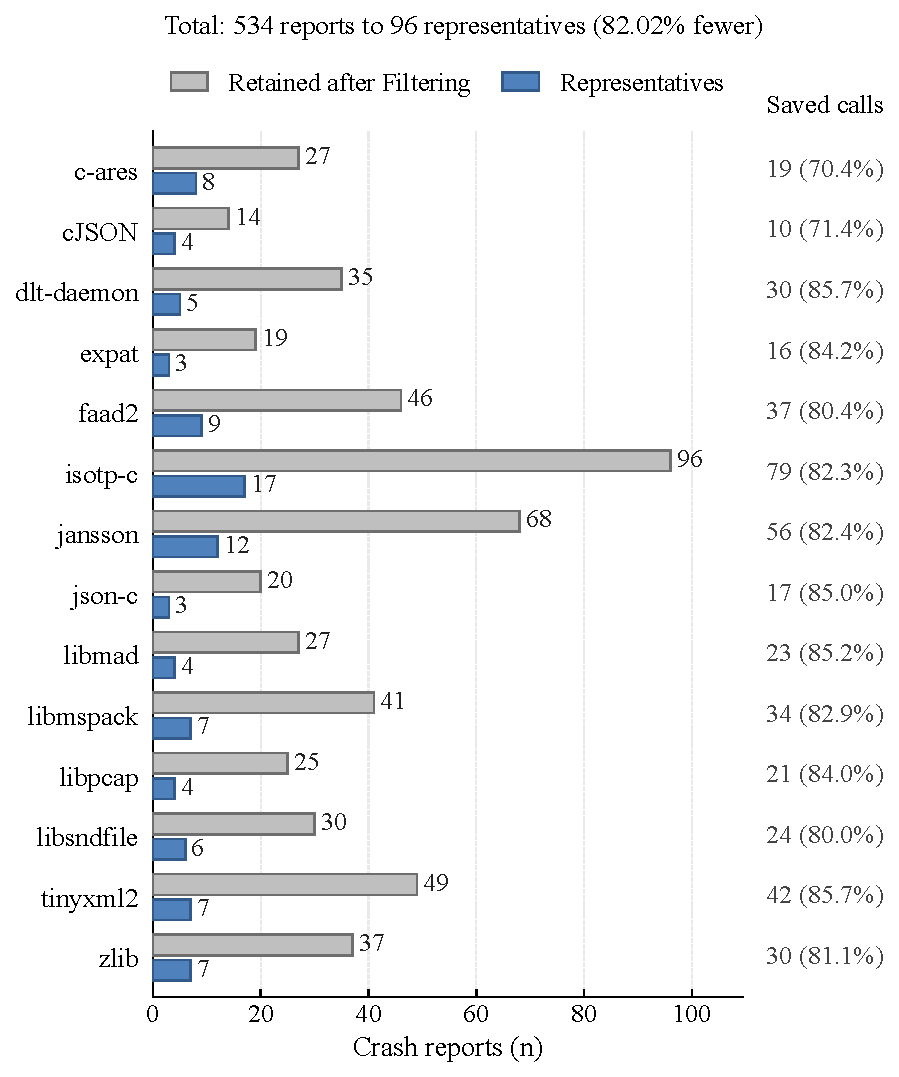
\includegraphics[width=0.75\linewidth]{figures/fig4.pdf}
\caption{Reduction in crash reports achieved by representative selection.}
\label{fig:representative-counts}
\end{figure}

Figure~\ref{fig:representative-counts} presents the reduction achieved by representative selection over the 95 reports retained after rule-guided crash attribution. Overall, only 21 of the 95 retained reports are submitted as representatives, removing 74 repeated or redundant reports.

These reductions combine two distinct effects. Rule-guided crash attribution first reduces the candidate set from 123 raw reports to 95 retained reports by filtering 28 reports, corresponding to a 22.8\% filtering reduction. On this retained set, representative selection keeps 21 representatives and removes 74 repeated or redundant reports, corresponding to a 77.9\% reduction in LLM submissions. Considering both rule-guided filtering and representative selection, the pipeline submits 21 representatives from the original 123 reports, reducing end-to-end LLM submissions by 82.9\%.

The reduction varies across components because the generated crashing inputs contain different levels of repetition. The larger reductions for c-ares and libpcap indicate that many retained reports share identical or similar stack signatures and can reuse the result of one representative. The smaller reduction for zlib indicates greater diversity among its seven reports, so a larger proportion must be retained. RQ2 is reported once because it measures the number of reports submitted to LLM analysis, which is determined by CrashSage before external adjudication. In response to RQ2, rule-guided filtering first removes low-value or likely driver-induced reports, and representative selection then reduces repeated LLM analysis over the retained candidate set by keeping one report for each group of crashes with matching exact or stack signatures.

\subsection{Evaluation of Crash-Context Reconstruction}
\label{subsec:rq3-localization}

To evaluate crash-context reconstruction, we compare V2 and V3 on the same crash reports. Both variants use rule-guided crash attribution and representative selection, while only V3 includes crash-context reconstruction. With the adjudication criterion held fixed, this comparison isolates the effect of adding crash-context reconstruction to V2.

\begin{table}[ht]
\caption{Effect of crash-context reconstruction under different external adjudicators.}
\label{tab:context-effect-v2-v3}
\centering
\scriptsize
\setlength{\tabcolsep}{3.2pt}
\renewcommand{\arraystretch}{1.12}
\begin{tabular*}{\linewidth}{@{\extracolsep{\fill}}lcc|cc|cc}
\toprule
\textbf{External Adjudicator} & \textbf{V2 P} & \textbf{V3 P} & \textbf{V2 R} & \textbf{V3 R} & \textbf{V2 F1} & \textbf{V3 F1} \\
\midrule
GPT-5.5 & 0.111 & 0.143 & 1.000 & 1.000 & 0.200 & 0.250 \\
Opus 4.8 & 0.111 & 0.143 & 0.333 & 0.333 & 0.167 & 0.200 \\
Kimi-2.7-Coder & 0.222 & 0.286 & 0.200 & 0.200 & 0.211 & 0.235 \\
Qwen3.7-Max & 0.222 & 0.286 & 0.667 & 0.667 & 0.333 & 0.400 \\
\botrule
\end{tabular*}
\end{table}

The experimental results are shown in Table~\ref{tab:context-effect-v2-v3}. V3 improves precision and F1 over V2 for all four adjudicators while preserving the same recall values.

This improvement is associated with the localization evidence added by crash-context reconstruction. A crash may become visible inside a target-component API even when the faulty state originates from the generated driver. Static code context links the visible crash site to the driver-to-component call path, while runtime context records the state observed during execution. In response to RQ3, these static and runtime evidence sources help adjudicators distinguish the visible crash location from the origin of the faulty state, matching the observed precision and F1 gains in Table~\ref{tab:context-effect-v2-v3} under the same conservative attribution setting.


\FloatBarrier

\subsection{Case Studies}
\label{subsec:case-studies}

To complement the quantitative results above, we present three case studies that illustrate how CrashSage prepares structured crash evidence before final LLM analysis.
They are selected to match the three evaluation concerns studied above: false-alert judgment, efficiency, and crash localization.
Table~\ref{tab:case-study-evidence} summarizes three case studies corresponding to the three evaluation concerns.

\begin{table}[ht]
\caption{Case studies for CrashSage evaluation}
\label{tab:case-study-evidence}
\centering
\compacttable
\setlength{\tabcolsep}{2.6pt}
\renewcommand{\arraystretch}{1.12}
\begin{tabularx}{\linewidth}{L{0.15\linewidth} Y Y Y}
\toprule
\textbf{Evidence} &
\textbf{Case 1: False-alert judgment} &
\textbf{Case 2: Efficiency} &
\textbf{Case 3: Crash localization} \\
\midrule
\textbf{Crash report}
& cJSON \texttt{driver\_4\_crash\_1}
& libpcap \texttt{driver\_15/27/29} group
& c-ares \texttt{driver\_18\_crash\_1} \\
\midrule
\textbf{Failure identity}
& \texttt{heap-buffer-overflow}
& repeated \texttt{libFuzzer: timeout}
& \texttt{SEGV} wild read \\
\midrule
\textbf{Attribution evidence}
& top crashing frame: driver
& shared \texttt{dedup\_token} / stack signature
& \texttt{ares\_init.c:520}; address \texttt{0xa01fa020} \\
\midrule
\textbf{Context or mapping}
& 20-byte driver heap region
& duplicate--representative pair; 5+ reports
& driver lines 28/36; replay 3/3 with registers \\
\midrule
\textbf{Pipeline output}
& \texttt{likely\_driver\_bug}; filtered
& duplicate skipped; representative reused
& runtime-context-supported diagnosis \\
\botrule
\end{tabularx}
\end{table}

In Case 1, the sanitizer reports a \texttt{heap-buffer-overflow}, but the top crashing frame and heap-boundary evidence are both confined to the generated driver.
The driver allocates a 20-byte \texttt{second\_str} buffer and then writes the terminator after copying fuzz input into that buffer, so the faulty state is created before any target-component behavior needs to be considered.
CrashSage therefore treats this report as \texttt{likely\_driver\_bug} and filters it before LLM analysis, illustrating how rule-guided attribution prevents a driver memory error from being counted as a target-component crash.

In Case 2, the libpcap reports form a repeated timeout group rather than independent failures.
The raw reports share the \texttt{libFuzzer: timeout} summary and the same timeout-oriented \texttt{dedup\_token}, and CrashSage records reports such as \texttt{driver\_27} and \texttt{driver\_29} as duplicates of the representative \texttt{driver\_15\_crash\_1} in a cluster of five or more reports.
Representative selection therefore skips duplicate LLM submissions and reuses the representative diagnosis, providing a concrete instance of the RQ2 result: redundant timeout reports are collapsed by signature evidence before final analysis.

In Case 3, the sanitizer reports a \texttt{SEGV} wild read at address \texttt{0x0000a01fa020}, with the project frame mapped to \texttt{ares\_init.c:520} in \texttt{init\_by\_options}.
The reconstructed driver context maps the failure back to line 28, where raw fuzz bytes are copied into a \texttt{struct ares\_options}, and line 36, where that structure is passed to \texttt{ares\_init\_options}.
Runtime replay reproduced the crash in all three attempts and recorded register evidence around the failing address, including \texttt{rax}/\texttt{rbx}=\texttt{0xa01fa020}, \texttt{rdx}=\texttt{0x28}, and the stack sequence \texttt{\_\_asan\_memcpy} $\rightarrow$ \texttt{ares\_init\_options} $\rightarrow$ \texttt{LLVMFuzzerTestOneInput}.
The final diagnosis therefore uses both the raw crash report and the reconstructed runtime context to identify an invalid callback or function-pointer state in \texttt{ares\_options}, rather than relying on the visible project frame alone.

\FloatBarrier

\section{Limitations}
\label{sec:limitations}

CrashSage is evaluated on four open-source components that correspond to common dependency roles in connected-vehicle software stacks, including DNS resolution, JSON processing, packet capture, and compression. These components provide representative supply-chain scenarios, but they do not cover all forms of automotive software. Components with properties such as real-time constraints or highly stateful protocol interactions may expose different crash patterns and API-usage assumptions. Therefore, the current evaluation mainly supports the applicability of CrashSage to open-source component-level fuzzing, while broader in-vehicle generalization requires additional component categories.

The current implementation follows one LLM-assisted fuzz-driver generation workflow and uses ASan+UBSan instrumentation. This setting is consistent across all evaluated variants, which keeps the comparison controlled, but other driver generators, prompt strategies, fuzzing engines, or sanitizer configurations may change the proportion of driver-induced crashes, duplicate reports, and target-component candidates. Extending CrashSage to additional driver-generation workflows and sanitizer combinations is left as future work.

Crash-context reconstruction also depends on replaying the crashing input and collecting runtime state in a stable execution environment. When replay fails or the reproduced crash does not match the original signature, CrashSage falls back to the normalized crash report and static context, which may reduce localization confidence. CrashSage is designed to reduce triage workload by filtering low-value reports, identifying driver-induced crashes, and submitting only retained representative reports to LLM analysis. Its use is therefore most appropriate as an evidence-preparation and attribution aid: it preserves reports that warrant further analysis and records the evidence used for each filtering or retention decision.

\FloatBarrier

\section{Conclusion}
\label{sec:conclusion}

CrashSage introduces an evidence-guided crash-adjudication pipeline for LLM-assisted fuzzing workloads. By applying rule-guided crash attribution, representative selection, and crash-context reconstruction before final LLM analysis, it replaces direct reasoning over raw crash reports with analysis over filtered, representative, and reconstructed crash evidence. In particular, representative selection reduces repeated crash instances before LLM analysis, and crash-context reconstruction combines static code context with replay-consistent runtime context for the selected representatives to distinguish the visible crash site from the origin and propagation of the faulty state. Evaluation on 123 crash reports from four open-source components shows that CrashSage improves crash attribution under the four external adjudicators. The full pipeline reduces end-to-end LLM submissions from 123 to 21 (82.9\%), with representative selection reducing the retained candidate set from 95 to 21 (77.9\%). Rule-guided crash attribution and representative selection each require less than 10 ms per report, whereas crash-context reconstruction requires approximately 2--15 s and LLM analysis requires approximately 30--60 s per case. These results demonstrate that CrashSage improves attribution quality while substantially reducing redundant LLM submissions. Future work will extend the evaluation to broader automotive component categories, additional driver-generation workflows, and more diverse sanitizer configurations.

\backmatter

% \bmhead{Acknowledgements}

% Not applicable.

% \bmhead{Author Contributions}

% Gaoqing Guan contributed to conceptualization, methodology, implementation, evaluation, and writing of the original draft. Tianqi Wu and Ying Zhang contributed to validation, result analysis, and manuscript review and editing. All authors read and approved the final manuscript.

% \bmhead{Funding}

% Not applicable.

% \bmhead{Data Availability}

% The data supporting the findings of this study are available from the corresponding author upon reasonable request.

% \section*{Declarations}

% \bmhead{Conflict of interest}

% The authors declare that they have no known competing financial interests or personal relationships that could have appeared to influence the work reported in this paper.

% ================= References =================
\bibliography{sn-bibliography}

\end{document}
